% article example for classicthesis.sty
\documentclass[11pt,a4paper]{scrartcl} % KOMA-Script article 
\usepackage{lipsum}
\usepackage{url}
\usepackage[LabelsAligned]{currvita} % nice cv style
\usepackage[nochapters]{classicthesis} % nochapters
\usepackage{tikz}
\usepackage{amsthm}
\usepackage{setspace}
\usepackage{pifont}
\usepackage{color}
\usepackage{graphicx}
\usetikzlibrary{calc,shapes,arrows,automata,trees,shadows,decorations.pathmorphing,positioning,
shapes.misc,shapes.arrows,chains,matrix,scopes,decorations.pathmorphing,backgrounds}
\renewcommand*{\cvheadingfont}{\LARGE\color{Maroon}}
\renewcommand*{\cvlistheadingfont}{\large}
\renewcommand*{\cvlabelfont}{\qquad}
\DeclareGraphicsExtensions{.pdf,.png,.jpg}
\begin{document}
\pagecolor{Sepia!04}
%Coverletter
\begin{cv}{\spacedallcaps{Child}}
        \begin{cvlist}{\textcolor{brown}{\spacedlowsmallcaps{Jason~N~Mansfield}}}\label{PersDat}  
            \item   Regis University
            \item   3333\\
                    Regis Boulevard Denver \\	
                    Colorado 80221-1099
            \item   mansf843@regis.edu\\				
                    \url{http://www.regis.edu/}				
        \end{cvlist}
        \begin{cvlist}{\spacedlowsmallcaps{RC~471}}\label{irgendwas}
            \item Instructed by Professor~Henri~Tshibambe\\
             \url{http://tinyurl.com/3htorkr}
        \end{cvlist}
    \end{cv}
\clearpage
\noindent
\begin{center}
\textcolor{Maroon}{\spacedallcaps{NIV Archaeological Study Bible~\cite{niv}}}\\
\textcolor{brown}{\spacedlowsmallcaps{Philippians~2}}
\end{center}
\begin{verse}
6 Who, being in very nature God, \\ did not consider equality with God \\ something to be grasped, 
\end{verse}
\begin{verse}
7 but made himself nothing,\\ taking the very nature of a\\ servant, \\ being made in human likeness.
\end{verse}
\begin{verse}
8 And being found in appearance as\\ a man,\\he humbled himself\\ and became obedient to death —\\ even death on a cross!
\end{verse}
\begin{verse}
9 Therefore God exalted him† to the\\ highest place\\ and gave him the name that is above\\ every name,
\end{verse}
\begin{verse}
10 that at the name of Jesus every\\ knee should bow,\\ in heaven and on earth and under\\ the earth,
\end{verse}
\begin{verse}
11 and every tongue confess that Jesus Christ is Lord,\\ to the glory of God the Father.
\end{verse} 
\clearpage
%Title
\title{\textcolor{Maroon}{\rmfamily\normalfont\spacedallcaps{Child}}}
    \author{\textcolor{brown}{\spacedlowsmallcaps{Jason N Mansfield}}}
    \date{} % no date
    
    \maketitle
    
    \begin{abstract}
Both my wife and I were raised in what could be considered extreme religous branches or to some even cults. Many of the mainstream religouns today were also considered cults themselves at one point in time, including Christianity itself as it branched from the standard Hebrew faith. My life and my goals have been shaped by my religon of the past and current. Doctrinal differences and bad choices put me in darkness for a portion of my life. Study and prayer allowed me to come back into the light. This essay outlines who I am today and why.
    \end{abstract}
       
    \tableofcontents

\section{Childhood}
\begin{figure}
\centering
\caption{Portion of the Dead Sea Scrolls}
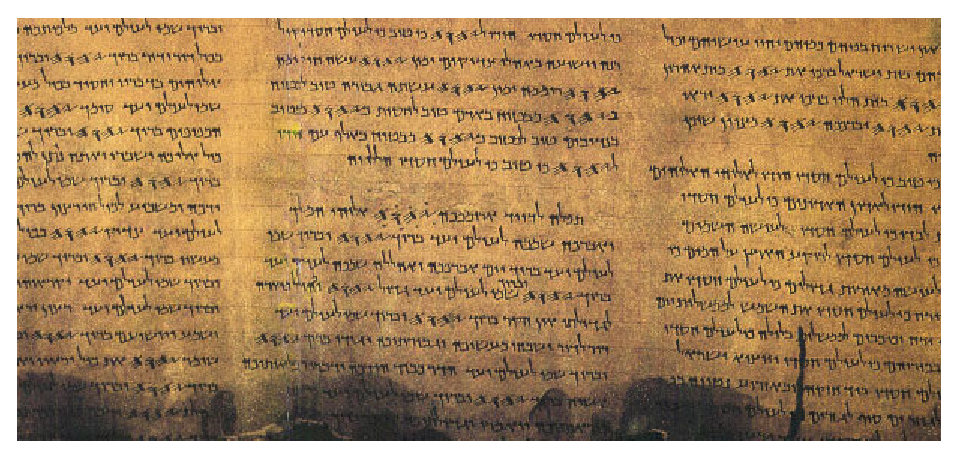
\includegraphics[scale=.50]{deadsea}
\end{figure}
\begin{doublespace}
\subsection{Jason's Childhood}
When I was very young my parents began teaching me to read. I would spend a large portion of my time reading from the bible due to the frequency of our studies. My mother also at an early age would read the bible but did not become a Jehovah's Witness~\cite{wiki:001} until near her teenage years. My father on the other hand went to more Mainline Protestant~\cite{wiki:003} type churches and converted later to become a Jehovah's Witness. Do to the rigorous readings each week I could read and write at a very early age as could my younger brother and sister. Being raised as a Jehovah's Witness was not horrible as some might imagine due to the lack of holiday's such as Christmas, Thanksgiving, Halloween, and others. I certainly had a strong understanding of the Bible and God's requirements of me. Looking back at my childhood now as a member of a Methodist Church~\cite{wiki:002} I am grateful for having parents who loved me enough to study the bible with me. Later on in life as I matured I began questioning certain teaching's by the Jehovah's Witnesses. The odd thing was it was usually the small questions that nagged at me, such as it being frowned upon to have a beared. While I had very little desire to grow a beard it bothered me that we could not grow one due to the strict standards set. Certainly Jesus is shown in all Jehovah's Witness literature as having a beard. However, while I belive this to be one area where the Jehovah's Witnesses have missed the mark, I also believe they are acurate in other areas. Regardless, of my beliefs in contrast to the Jehovah's Witnesses I believe all orginized relgions have their inherent mistakes and accomplishments. 
\subsection{April's Childhood}
My wife and I have discussed her upbringing and the faith she was introduced to while at a young age many times. April's father began his own church in the form of Non-denominational Christianity~\cite{wiki:004} which considers itself to be a spirit filled church or one that encorages the practice of Glossolalia~\cite{wiki:005}. At a young age my wife agreed with her fathers teachings but as she matured she began to disapprove of certain practices and docrtinal beliefs. Similar to my experience in life my wife began to lose her faith due to conflict with her true beliefs and the religous structure formed around her. 
\end{doublespace}
\begin{center}
\textcolor{Maroon}{\spacedallcaps{NIV Archaeological Study Bible~\cite{niv}}}\\
\textcolor{brown}{\spacedlowsmallcaps{John~12}}\\
\end{center}
\begin{verse}
35 Then Jesus told them, “You are going to have the light† just a little while longer. Walk while you have the light,† before darkness overtakes you.† The man who walks in the dark does not know where he is going.
\end{verse}
\begin{verse}
 36 Put your trust in the light while you have it, so that you may become sons of light.”† When he had finished speaking, Jesus left and hid himself from them.† 
\end{verse}

\section{Into Darkness}
\begin{doublespace}
\subsection{Decent}
One Autumn in Maine my family faced a series of trageties all in sequence, my parents divorce, our house burning down, my younger brothers accidental death. It all came relentlessly and for someone sheltered by a tighly knit community where nothing bad ever happened it was unbearable. My brother had previously been absent from the Jehovah's Witness Congregation and to some degree considered bad news due to his recent lifestyle. I had assumed that members of this orginization would still have some concern considering they watched my brother grow up since a baby. While I can't be certain that I was not already being drawn away from the Jehovah's Witnesses by my own doubts, the fact that this particular group did nothing to aid our family during this time seemed opposite to their claims of brotherhood. Once again I cannot claim to understand everyones intensions. It is possible some of the members made efforts during our bad period but I was not made aware. Without placing blame on the Jehovah's Witness orginization as a whole I am well aware that I allowed myself to slip into a spiritual coma. 
\subsection{Wrong choices}
I had written religion off and stopped praying all together. I was filled with bitterness and felt betrayed. I rebeled completely and unthinkingly. Not only was I headed down a dark road but so were all my closest friends who were also close to my brother. We began spending our days plotting on getting drunk and partying. My goals were gone and I had no motivation and no heros left. For all intensive purposes I was dead inside. The next few years were a painful blurr of wasted time and alchoholic raging. I began associating with people even my worst friends would accept company with. The pain of my brothers death only increased from this lifestyle. It got to the point where all I knew was misery and pain. 
\end{doublespace}
\begin{center}
\textcolor{Maroon}{\spacedallcaps{NIV Archaeological Study Bible~\cite{niv}}}\\
\textcolor{brown}{\spacedlowsmallcaps{John~12}}\\
\end{center}
\begin{verse}
44 Then Jesus cried out, “When a man believes in me, he does not believe in me only, but in the one who sent me.
\end{verse}
\begin{verse}
45 When he looks at me, he sees the one who sent me.
\end{verse}
\begin{verse}
 46 I have come into the world as a light,† so that no one who believes in me should stay in darkness. 
\end{verse}
\section{The Light}
\begin{doublespace}
\subsection{Surfs Up}
One winters day while I was still living in the College town of Orono Maine one of my closest friends called me from the Outer Banks of North Carolina talking about long beautiful golden beaches, surfing and a new lifestyle. Within a month I had driven down to Kitty Hawk, NC and moved into a home with him and his fiancee. While I was still not praying or attempting to approach God, this move away from my bad lifestyle may have saved my life. I spent the next two years surfing, swimming and begining to see the value of life again. 
\subsection{The Navy}
Three years later after scrapping back up what used to be my original personality I was abile to put my life back into drive. Due to my dropping out of college I decided to scrap up what oportunities I had left and joined the Navy. This was somthing that was not allowed when a Jehovah's Witness but I was so far away from my original teaching now that I no longer cared. After my first tour in the Persian Gulf on the USS John F. Kennedy (CV-67)~\cite{wiki:006} with my Command VFA-81~\cite{wiki:007} I left the Navy a better person. I had certainly experienced some miserable and possible dangerous days in the Navy but I am thankful for the opportunities my service created for me. 
\end{doublespace}
\begin{center}
\textcolor{Maroon}{\spacedallcaps{NIV Archaeological Study Bible~\cite{niv}}}\\
\textcolor{brown}{\spacedlowsmallcaps{Romans~14}}\\
\end{center}
\begin{verse}
11 And do this, understanding the present time. The hour has come† for you to wake up from your slumber,† because our salvation is nearer now than when we first believed. 
\end{verse}
\begin{verse}
12 The night is nearly over; the day is almost here.† So let us put aside the deeds of darkness† and put on the armor† of light.
\end{verse}
\begin{verse}
13 Let us behave decently, as in the daytime, not in orgies and drunkenness, not in sexual immorality and debauchery, not in dissension and jealousy.† 
\end{verse}
\begin{verse}
14 Rather, clothe yourselves with the Lord Jesus Christ,† and do not think about how to gratify the desires of the sinful nature.
\end{verse}
\section{April}
\subsection{Communications Class}
\begin{doublespace}
Once I left the Navy I immediatly knew I wanted to pursue a career in Computer Science. When I wasnt surfing I was modifying my computer and writing randoms scripts for linux based software. My hobby had gotten to the point where I knew it could be a real career move. I began attending classes at ECPI University in Norfolk, VA. My life was looking up and I was no loger bogged down by guilt, bad habbits, or the pain I had experienced daily years before. Somthing was still missing in my life. I felt a hollowness. I began to slowly pray again. At first I felt insane as if I was praying to the wall or talking to myself. I had doubts that I was simply programmed by my previous religion to believe in God and that I was a crazy person speaking to myself. One night while praying for forgiveness for all my sins and began to ask God for someone in my life who loves him. The next day I met my future wife April a Pastors daughter. 
\subsection{Methodist Church}
There is not a day that goes by that I don't thank God for all that he has given me. In a few short years since my prayer I have been blessed with a beautiful motivated faithful wife and three boys. My wife and I both come from very versitile religous groups. I am careful not to claim either group is dead wrong in their doctrins or that our beliefs are better. What I do believe is that each man and woman need create their own covenent with God and honor it. The Methodist church has and will continue to serve as a safe haven for my family.
\subsection{The future}
I would not claim that I made progress to get where I am today but that God has placed me here. I await his direction but I'm not stagnating and waiting for propmts or miracles. I follow my parents example and study the bible with my children. We attend my wifes fathers church to show respect from time to time and the same for my mother. I do not claim to be a saint but I do have spiritual goals. My wife and I try to stay active with our church and plan to make valid efforts to be more involved in the future with extra events. I always take the opportunity to invite others to go and enjoy this gathering with us. Beyond, my life at church I intend to do furthur research constantly educating myself and working towards both a spiritual enlightenment and educational one. Reading books by author Gerald L. Schroeder~\cite{gerald-2009} has helped me tremedously in increasing my faith to new heights. Life still offers it's challenges but with my previous experiences I am very content with having a clean home, dependable vehicles, an amazing wife and three beautiful boys. I am truly thankful for all God have given me. I do not intend to squander those gifts. While I go through life I will base my success on the spiritual foundation I create for my children. I hope that through teaching them to avoid some of the horrible mistakes I have made and following in Jesus footsteps I may approach him closer as well.

\end{doublespace}
\clearpage
  % bib stuff
    \nocite{*}
    \addtocontents{toc}{\protect\vspace{\beforebibskip}}
    \addcontentsline{toc}{section}{\refname}    
    \bibliographystyle{plain}
    \bibliography{cite}
\end{document}